% ----------------------------------------------------------------------------------------------------- %
% Manual da Classe UFTeX
% 
% Versão 2.1:   Março 2018
%
% Criado por:   Tiago da Silva Almeida
% Revisado por: Tiago da Silva Almeida
%               Rafael Lima de Carvalho
%               Ary Henrique Morais de Oliveira
%
% https://almeidatiago.github.io/uftex/
% ----------------------------------------------------------------------------------------------------- %
\documentclass[tcc1,project]{uftex}

\usepackage[alf,abnt-emphasize=bf]{abntex2cite}
\usepackage{booktabs}
\usepackage{geometry}
\usepackage{listings}
\usepackage{xcolor}
\geometry{a4paper, margin=1in}
\renewcommand{\backrefpagesname}{}
\renewcommand{\backref}{}
\renewcommand*{\backrefalt}[4]{}
\setcounter{section}{0}

\begin{document}
\setlength\parindent{15pt}


  \title{Análise dos Algoritmos de Ordenação}
  % \foreigntitle{Thesis Title}
  \author{Ícaro Mesquita e Kalil Garcia}{Canuto}


  \department{CC}
  \date{07}{10}{2024}

  \keyword{Algoritmo de Ordenação}
  \keyword{Análise de Algoritmos}
  

  \maketitle

  \begin{abstract}
\paragraph{}
Os algoritmos de ordenação desempenham um papel fundamental na ciência da computação, fornecendo métodos essenciais para organizar dados de forma eficiente. Este artigo explora diversos algoritmos de ordenação, incluindo Bubble Sort, Selection Sort, Insertion Sort, Merge Sort, Quick Sort e Heap Sort. Analisamos seu desempenho com base no tempo de execução, número de comparações e trocas, considerando diferentes cenários de entrada, como listas ordenadas, inversamente ordenadas e aleatórias. Por meio de uma análise empírica, destacamos os pontos fortes e fracos de cada algoritmo, demonstrando como sua eficiência pode variar dependendo das características dos dados processados. Os resultados enfatizam a importância de selecionar o algoritmo de ordenação adequado para otimizar o desempenho em diversas aplicações, desde bancos de dados até motores de busca. Em última análise, este estudo contribui para uma compreensão mais profunda da eficiência algorítmica e suas implicações práticas na gestão de dados.
 \end{abstract}


% ----------------------------------------------------------------------------------------------------- %
% Capítulos do trabalho
% ----------------------------------------------------------------------------------------------------- %
\chapter{Introdução}
\paragraph{}
A ordenação de dados é um dos pilares fundamentais na ciência da computação e em diversas aplicações práticas, desempenhando um papel crucial na eficiência de algoritmos e na gestão de informações. Em um mundo onde a quantidade de dados gerados está crescendo exponencialmente, a capacidade de organizar essas informações de maneira eficiente é vital. A ordenação não apenas facilita a busca e a recuperação de dados, mas também melhora a legibilidade e a análise, permitindo que os usuários tomem decisões informadas de maneira mais rápida. Como destacado por Leonel (2017), "a eficiência dos algoritmos é fundamental para garantir a performance em processos de ordenação".

Além disso, muitos algoritmos e estruturas de dados, como árvores de busca e tabelas hash, dependem de dados ordenados para funcionar de forma otimizada. A escolha do algoritmo de ordenação adequado pode impactar significativamente o desempenho de sistemas em aplicações como bancos de dados, motores de busca, e-commerce, e muito mais. Portanto, entender os diferentes métodos de ordenação e suas complexidades é essencial para o desenvolvimento de soluções eficientes que atendam às necessidades do mundo contemporâneo.

Neste artigo, iremos realizar a análise e a comparação do desempenho de diferentes algoritmos de ordenação em termos de eficiência, tempo de execução e número de operações (comparações e trocas). Em face do crescimento incessante do volume dos dados disponíveis, a escolha do algoritmo de ordenação apropriado torna-se fundamental para garantir eficiência e rapidez quando se trata de manipular informações. Este estudo busca fornecer uma compreensão prática de como diferentes algoritmos se comportam em diferentes condições, possibilitando que desenvolvedores e engenheiros de software tenham informações suficientes para elaborar suas escolhas em suas aplicações.

Algoritmos sujeitos à Análise

Para os efeitos deste trabalho, serão analisados os seguintes algoritmos de ordenação:

Bubble Sort: Um algoritmo simples, mas ineficaz para conjuntos extensos de dados. Sua principal característica está na troca sucessiva de elementos adjacentes.

Selection Sort: Um método que divide o vetor em duas partes, apesar de ordenar a primeira parte,arada a segunda parte, marcada como não ordenada, a seleção repetida do menor elemento da parte não ordenada.

Insertion Sort: Um algoritmo que constrói a ordenação final de uma lista através da construção um item de cada vez, inserindo cada nova medição na posição do que apresenta.

Merge Sort: Um algoritmo de divisão e conquista que divide a lista em sublistas menores, ordena as sublistas e em seguida, as mescla em lista ordenada. 

Quick Sort: Um método que para dividir a lista utiliza um elemento pivô, gerando duas sublistas e ordenando-as em uma forma recursiva.

Heap Sort: Um algoritmo que se utiliza da estrutura de dados heap para ordenar elementos, construindo um heap máximo e extraindo o maior elemento corrente repetidamente.

O exame destes algoritmos será realizado sob diversas condições, incluindo diversos tamanhos de entradas e distribuições dos dados (ordenados, inversamente ordenados e aleatórios), permitindo uma avaliação completa de seus desempenhos. 

\chapter{Revisão Teórica}
Devemos considerar, portanto os algoritmos que forama analisados sobre os critérios estabelecidos considerando padrões distintos de ordenação das listas e tamanhos também. Logo, temos 
\section{Bubble Sort}
O Bubble Sort é um dos algoritmos de ordenação mais simples. Ele funciona iterando pela lista, comparando elementos adjacentes e trocando-os se estiverem na ordem errada. Esse processo é repetido até que a lista esteja ordenada. \textit{in place}, mas não é estável. \\
\textbf{Complexidade:}
\begin{itemize}
    \item Melhor caso: $O(n)$ (quando a lista já está ordenada)
    \item Caso médio: $O(n^2)$
    \item Pior caso: $O(n^2)$
    
\end{itemize}
\textbf{Estabilidade:} Sim, mantém a ordem dos elementos iguais. \\
\textbf{In Place:} Sim, o Bubble Sort não requer espaço adicional significativo. \\

\section{Selection Sort}
O Selection Sort divide a lista em duas partes: a parte ordenada e a parte não ordenada. A cada iteração, o menor (ou maior, dependendo da ordem desejada) elemento da parte não ordenada é selecionado e movido para a parte ordenada. \\
\textbf{Complexidade:}
\begin{itemize}
    \item Melhor caso: $O(n^2)$
    \item Caso médio: $O(n^2)$
    \item Pior caso: $O(n^2)$
    
    
\end{itemize}
\textbf{Estabilidade:} Não, pois pode trocar elementos iguais, alterando sua ordem relativa. \\
\textbf{In Place:} Sim, o Selection Sort não requer espaço adicional significativo. \\

\section{Insertion Sort}
O Insertion Sort constrói a lista ordenada um elemento de cada vez, pegando cada novo elemento e inserindo-o na posição correta na parte já ordenada da lista. \\
\textbf{Complexidade:}
\begin{itemize}
    \item Melhor caso: $O(n)$ (quando a lista já está ordenada)
    \item Caso médio: $O(n^2)$
    \item Pior caso: $O(n^2)$
    
\end{itemize}
\textbf{Estabilidade:} Sim, mantém a ordem dos elementos iguais. \\
\textbf{In Place:} Sim, o Insertion Sort não requer espaço adicional significativo. \\

\section{Merge Sort}
O Merge Sort é um algoritmo baseado na técnica de divisão e conquista. Ele divide a lista em duas metades, ordena cada metade recursivamente e, em seguida, mescla as duas metades ordenadas. \\
\textbf{Complexidade:}
\begin{itemize}
    \item Melhor caso: $O(n \log n)$
    \item Caso médio: $O(n \log n)$
    \item Pior caso: $O(n \log n)$
    
\end{itemize}
\textbf{Estabilidade:} Sim, mantém a ordem dos elementos iguais. \\
\textbf{In Place:} Não, pois requer espaço adicional para armazenar as sublistas durante a mesclagem. \\

\section{Quick Sort}
O Quick Sort também utiliza a técnica de divisão e conquista. Ele escolhe um elemento como pivô e particiona a lista em torno do pivô, ordenando recursivamente as sublistas resultantes. \\
\textbf{Complexidade:}
\begin{itemize}
    \item Melhor caso: $O(n \log n)$
    \item Caso médio: $O(n \log n)$
    \item Pior caso: $O(n^2)$ (quando a lista já está ordenada ou inversamente ordenada, dependendo da escolha do pivô)
    
\end{itemize}
\textbf{Estabilidade:} Não, pois pode alterar a ordem relativa dos elementos iguais. \\
\textbf{In Place:} Sim, o Quick Sort geralmente é implementado como um algoritmo in-place. \\

\section{Heap Sort}
O Heap Sort utiliza a estrutura de dados heap para ordenar os elementos. Primeiro, ele constrói um heap máximo a partir da lista e, em seguida, extrai o maior elemento repetidamente, reconstruindo o heap até que todos os elementos estejam ordenados. \\
\textbf{Complexidade:}
\begin{itemize}
    \item Melhor caso: $O(n \log n)$
    \item Caso médio: $O(n \log n)$
    \item Pior caso: $O(n \log n)$
    
    
\end{itemize}
\textbf{Estabilidade:} Não, pois pode alterar a ordem relativa dos elementos iguais. \\
\textbf{In Place:} Sim, o Heap Sort não requer espaço adicional significativo. \\
\chapter{Metodologia}

\section{Descrição do Ambiente de Teste}
O ambiente de teste utilizado para realizar os experimentos com os algoritmos de ordenação consistiu no seguinte hardware e software:
\subsection{Hardware:}
\begin{itemize}
    \item Processador: AMD Ryzen 5-5500U
    \item Memória RAM: 8 GB DDR4
    \item Armazenamento: 256GB SSD PCie
\end{itemize}

\subsection{Software:}
\begin{itemize}
    \item Sistema Operacional: Fedora Linux versão 40
    \item Linguagem de Programação: Python 3.13.0rc2
    \item Bibliotecas Utilizadas:
        \begin{itemize}
            \item Matplotlib (para a visualização dos gráficos)
            \item Time (para medir o tempo de execução)
            \item Random (para a geração de listas aleatórias)
        \end{itemize}
\end{itemize}

Esse ambiente foi escolhido por fornecer recursos computacionais suficientes para executar os algoritmos com listas de tamanhos variados, garantindo resultados adequados em termos de desempenho e tempo de execução.

\section{Implementação dos Algoritmos}
Os algoritmos de ordenação foram implementados em Python e incluíram os seguintes métodos:
\begin{itemize}
    \item Bubble Sort
    \item Selection Sort
    \item Insertion Sort
    \item Merge Sort
    \item Quick Sort
    \item Heap Sort
\end{itemize}

Cada algoritmo foi adaptado para registrar o número de comparações e trocas durante o processo de ordenação, permitindo uma análise detalhada de sua eficiência em termos dessas métricas.

O código de cada algoritmo foi estruturado em classes, onde as comparações e trocas eram contabilizadas durante o processo de ordenação. Abaixo estão os exemplos e explicações para cada algoritmo:

\subsection{Bubble Sort}
O algoritmo Bubble Sort compara elementos adjacentes de uma lista e os troca caso estejam na ordem incorreta. Isso é repetido até que a lista esteja ordenada. Ele é conhecido por sua simplicidade, mas é um dos algoritmos menos eficientes em termos de tempo.

\begin{lstlisting}[language=Python, caption=BubbleSort]
class BubbleSort:
    def __init__(self, arr):
        self.arr = arr
        self.comparisons = 0
        self.swaps = 0

    def sort(self):
        for i in range(len(self.arr)):
            for j in range(len(self.arr) - 1):
                self.comparisons += 1
                if self.arr[j] > self.arr[j + 1]:
                    self.arr[j], self.arr[j + 1] = self.arr[j + 1], self.arr[j]
                    self.swaps += 1
        return self.arr, self.comparisons, self.swaps
\end{lstlisting}

\subsection{Selection Sort}
O algoritmo Selection Sort encontra o menor elemento da lista e o coloca na posição correta. Ele repete esse processo para os subarrays restantes até que a lista esteja ordenada. Embora mais eficiente que o Bubble Sort, ainda não é a melhor opção para grandes listas.

\begin{lstlisting}[language=Python, caption=SelectionSort]
class SelectionSort:
    def __init__(self, arr):
        self.arr = arr
        self.comparisons = 0
        self.swaps = 0
    
    def sort(self):
        for i in range(len(self.arr)):
            min_index = i
            for j in range(i + 1, len(self.arr)):
                self.comparisons += 1
                if self.arr[j] < self.arr[min_index]:
                    min_index = j
            if min_index != i:
                self.arr[i], self.arr[min_index] = self.arr[min_index], self.arr[i]
                self.swaps += 1
        return self.arr, self.comparisons, self.swaps
\end{lstlisting}

\subsection{Insertion Sort}
O Insertion Sort constrói a lista ordenada de forma incremental, movendo um elemento por vez para sua posição correta. Ele é mais eficiente que o Bubble e o Selection Sort em listas quase ordenadas.

\begin{lstlisting}[language=Python, caption=InsertionSort]
class InsertionSort:
    def __init__(self, arr):
        self.arr = arr
        self.comparisons = 0
        self.swaps = 0

    def sort(self):
        for i in range(1, len(self.arr)):
            key = self.arr[i]
            j = i - 1
            while j >= 0:
                self.comparisons += 1
                if key < self.arr[j]:
                    self.arr[j + 1] = self.arr[j]
                    self.swaps += 1
                    j -= 1
                else:
                    break
            self.arr[j + 1] = key
        return self.arr, self.comparisons, self.swaps
\end{lstlisting}

\subsection{Merge Sort}
O Merge Sort é um algoritmo de ordenação baseado no paradigma "Dividir para Conquistar". Ele divide a lista em sublistas menores, ordena essas sublistas e as combina para formar a lista ordenada. Ele é mais eficiente que os anteriores, com complexidade $O(n \log n)$.

\begin{lstlisting}[language=Python, caption=MergeSort]
class MergeSort:
    def __init__(self, arr):
        self.arr = arr
        self.comparisons = 0
        self.assignments = 0

    def merge_sort(self, arr=None):
        if arr is None:
            arr = self.arr

        if len(arr) > 1:
            mid = len(arr) // 2
            left_half = arr[:mid]
            right_half = arr[mid:]

            self.merge_sort(left_half)
            self.merge_sort(right_half)

            i = j = k = 0

            while i < len(left_half) and j < len(right_half):
                self.comparisons += 1
                if left_half[i] < right_half[j]:
                    arr[k] = left_half[i]
                    self.assignments += 1
                    i += 1
                else:
                    arr[k] = right_half[j]
                    self.assignments += 1
                    j += 1
                k += 1

            while i < len(left_half):
                arr[k] = left_half[i]
                self.assignments += 1
                i += 1
                k += 1

            while j < len(right_half):
                arr[k] = right_half[j]
                self.assignments += 1
                j += 1
                k += 1

    def sort(self):
        self.merge_sort()
        return self.arr, self.comparisons, self.assignments
\end{lstlisting}

\subsection{Quick Sort}
O Quick Sort também utiliza o paradigma "Dividir para Conquistar", escolhendo um elemento como pivô e particionando a lista ao redor desse pivô. Apesar de sua complexidade $O(n \log n)$, pode ser ineficiente em alguns casos, como listas quase ordenadas, sem um bom pivô.

\begin{lstlisting}[language=python, caption=QuickSort]
class QuickSort:
    def __init__(self, arr):
        self.arr = arr
        self.comparisons = 0
        self.swaps = 0

    def quick_sort(self):
        self._quick_sort_helper(0, len(self.arr) - 1)

    def _quick_sort_helper(self, low, high):
        if low < high:
            pivot_index = self._partition(low, high)
            self._quick_sort_helper(low, pivot_index - 1)
            self._quick_sort_helper(pivot_index + 1, high)

    def _partition(self, low, high):
        random_pivot = random.randint(low, high)
        self.arr[high], self.arr[random_pivot] = self.arr[random_pivot], self.arr[high]
        self.swaps += 1

        pivot = self.arr[high]
        i = low - 1

        for j in range(low, high):
            self.comparisons += 1
            if self.arr[j] <= pivot:
                i += 1
                self.arr[i], self.arr[j] = self.arr[j], self.arr[i]
                self.swaps += 1

        self.arr[i + 1], self.arr[high] = self.arr[high], self.arr[i + 1]
        self.swaps += 1
        return i + 1

    def sort(self):
        self.quick_sort()
        return self.arr, self.comparisons, self.swaps
\end{lstlisting}

\subsection{Heap Sort}
O Heap Sort transforma a lista em uma estrutura de heap e extrai o maior elemento sucessivamente, colocando-o no final da lista. Sua complexidade também é $O(n \log n)$, e ele é eficiente tanto em tempo quanto em espaço.

\begin{lstlisting}[language=Python, caption=HeapSort]
class HeapSort:
    def __init__(self, arr):
        self.arr = arr
        self.comparisons = 0
        self.swaps = 0

    def heap_sort(self):
        n = len(self.arr)

        for i in range(n // 2 - 1, -1, -1):
            self._heapify(n, i)

        for i in range(n - 1, 0, -1):
            self.arr[i], self.arr[0] = self.arr[0], self.arr[i]
            self.swaps += 1
            self._heapify(i, 0)

    def _heapify(self, n, i):
        largest = i
        left = 2 * i + 1
        right = 2 * i + 2

        if left < n:
            self.comparisons += 1
            if self.arr[i] < self.arr[left]:
                largest = left

        if right < n:
            self.comparisons += 1
            if self.arr[largest] < self.arr[right]:
                largest = right

        if largest != i:
            self.arr[i], self.arr[largest] = self.arr[largest], self.arr[i]
            self.swaps += 1
            self._heapify(n, largest)

    def sort(self):
        self.heap_sort()
        return self.arr, self.comparisons, self.swaps
\end{lstlisting}

A implementação de todos os algoritmos seguiu esse formato


\definecolor{codeblue}{rgb}{0.26, 0.42, 0.96}
\definecolor{codegreen}{rgb}{0.0, 0.5, 0.0}
\definecolor{codegray}{rgb}{0.5, 0.5, 0.5}
\definecolor{backcolour}{rgb}{0.95, 0.95, 0.92}

\lstdefinestyle{mystyle}{
    backgroundcolor=\color{backcolour},   
    commentstyle=\color{codegreen},
    keywordstyle=\color{codeblue},
    numberstyle=\tiny\color{codegray},
    stringstyle=\color{codeblue},
    basicstyle=\ttfamily\footnotesize,
    breakatwhitespace=false,         
    breaklines=true,                 
    captionpos=b,                    
    keepspaces=true,                 
    numbers=left,                    
    numbersep=5pt,                  
    showspaces=false,                
    showstringspaces=false,
    showtabs=false,                  
    tabsize=2
}

\lstset{style=mystyle}

\chapter{Resultados}
\section{Tabelas}
Neste capítulo, apresentaremos os resultados obtidos a partir dos testes realizados com os algoritmos de ordenação. Os resultados serão apresentados por meio de tabelas e gráficos comparativos, destacando o desempenho de cada algoritmo em termos de tempo de execução, número de comparações, e número de trocas. As análises serão feitas considerando diferentes tamanhos de listas (1.000, 10.000, 50.000 e 100.000 elementos) e três distribuições de dados: listas aleatórias, ordenadas, e inversamente ordenadas.

\begin{table}[h]
\centering
\caption{Resultados do Bubble Sort para diferentes tamanhos e tipos de lista}
\begin{tabular}{llrrr}
\toprule
\textbf{Tamanho} & \textbf{Tipo de Lista} & \textbf{Comparações} & \textbf{Tempo (ms)} & \textbf{Trocas} \\
\midrule
\multirow{3}{*}{1,000}   & Ordem Aleatória   & 999,000  & 50.431    & 243,786 \\
                         & Ordem Crescente   & 999,000  & 36.4013   & 0 \\
                         & Ordem Decrescente & 999,000  & 59.7439   & 499,500 \\
\midrule
\multirow{3}{*}{10,000}  & Ordem Aleatória   & 99,990,000  & 5,134.17   & 25,020,403 \\
                         & Ordem Crescente   & 99,990,000  & 3,818.43   & 0 \\
                         & Ordem Decrescente & 99,990,000  & 6,176.45   & 49,995,000 \\
\midrule
\multirow{3}{*}{50,000}  & Ordem Aleatória   & 2,499,950,000  & 136,715  & 624,472,556 \\
                         & Ordem Crescente   & 2,499,950,000  & 101,897  & 0 \\
                         & Ordem Decrescente & 2,499,950,000  & 164,154  & 1,249,975,000 \\
\midrule
\multirow{3}{*}{100,000} & Ordem Aleatória   & 9,999,900,000  & 574,547  & 2,500,274,308 \\
                         & Ordem Crescente   & 9,999,900,000  & 426,037  & 0 \\
                         & Ordem Decrescente & 9,999,900,000  & 691,768  & 4,999,950,000 \\
\bottomrule
\end{tabular}
\end{table}


\begin{table}[h]
\centering
\caption{Resultados do Merge Sort para diferentes tamanhos e tipos de lista}
\begin{tabular}{llrrr}
\toprule
\textbf{Tamanho} & \textbf{Tipo de Lista} & \textbf{Comparações} & \textbf{Tempo (ms)} & \textbf{Trocas} \\
\midrule
\multirow{3}{*}{1,000}   & Ordem Aleatória   & 8,682   & 799.179   & 0 \\
                         & Ordem Crescente   & 4,932   & 620.842   & 0 \\
                         & Ordem Decrescente & 5,044   & 612.020   & 0 \\
\midrule
\multirow{3}{*}{10,000}  & Ordem Aleatória   & 120,508 & 10,561.0  & 0 \\
                         & Ordem Crescente   & 64,608  & 8,030.89  & 0 \\
                         & Ordem Decrescente & 69,008  & 8,079.05  & 0 \\
\midrule
\multirow{3}{*}{50,000}  & Ordem Aleatória   & 717,919 & 62,367.0  & 0 \\
                         & Ordem Crescente   & 382,512 & 45,893.0  & 0 \\
                         & Ordem Decrescente & 401,952 & 46,651.1  & 0 \\
\midrule
\multirow{3}{*}{100,000} & Ordem Aleatória   & 1,536,678 & 132,979.0 & 0 \\
                         & Ordem Crescente   & 815,024   & 97,579.7  & 0 \\
                         & Ordem Decrescente & 853,904   & 98,982.1  & 0 \\
\bottomrule
\end{tabular}
\end{table}


\begin{table}[h]
\centering
\caption{Resultados do Selection Sort para diferentes tamanhos e tipos de lista}
\begin{tabular}{llrrr}
\toprule
\textbf{Tamanho} & \textbf{Tipo de Lista} & \textbf{Comparações} & \textbf{Tempo (ms)} & \textbf{Trocas} \\
\midrule
\multirow{3}{*}{1,000}   & Ordem Aleatória   & 499,500  & 15.8987   & 993 \\
                         & Ordem Crescente   & 499,500  & 15.7552   & 0 \\
                         & Ordem Decrescente & 499,500  & 16.2408   & 500 \\
\midrule
\multirow{3}{*}{10,000}  & Ordem Aleatória   & 49,995,000  & 1,579.78   & 9,991 \\
                         & Ordem Crescente   & 49,995,000  & 1,542.77   & 0 \\
                         & Ordem Decrescente & 49,995,000  & 1,591.73   & 5,000 \\
\midrule
\multirow{3}{*}{50,000}  & Ordem Aleatória   & 1,249,975,000  & 40,428.0  & 49,990 \\
                         & Ordem Crescente   & 1,249,975,000  & 38,464.0  & 0 \\
                         & Ordem Decrescente & 1,249,975,000  & 40,833.1  & 25,000 \\
\midrule
\multirow{3}{*}{100,000} & Ordem Aleatória   & 4,999,950,000  & 177,423.0 & 99,986 \\
                         & Ordem Crescente   & 4,999,950,000  & 170,632.0 & 0 \\
                         & Ordem Decrescente & 4,999,950,000  & 176,048.0 & 50,000 \\
\bottomrule
\end{tabular}
\end{table}

\begin{table}[h]
\centering
\caption{Resultados do Heap Sort para diferentes tamanhos e tipos de lista}
\begin{tabular}{llrrr}
\toprule
\textbf{Tamanho} & \textbf{Tipo de Lista} & \textbf{Comparações} & \textbf{Tempo (ms)} & \textbf{Trocas} \\
\midrule
\multirow{3}{*}{1,000}   & Ordem Aleatória   & 16,849  & 1.44005   & 9,076 \\
                         & Ordem Crescente   & 17,583  & 1.48201   & 9,708 \\
                         & Ordem Decrescente & 15,965  & 1.29199   & 8,316 \\
\midrule
\multirow{3}{*}{10,000}  & Ordem Aleatória   & 235,411  & 20.0591   & 124,198 \\
                         & Ordem Crescente   & 244,460  & 20.9391   & 131,956 \\
                         & Ordem Decrescente & 226,682  & 18.7342   & 116,696 \\
\midrule
\multirow{3}{*}{50,000}  & Ordem Aleatória   & 1,409,625  & 118.528  & 737,403 \\
                         & Ordem Crescente   & 1,455,438  & 121.738  & 773,304 \\
                         & Ordem Decrescente & 1,366,047  & 110.084  & 698,892 \\
\midrule
\multirow{3}{*}{100,000} & Ordem Aleatória   & 3,019,690  & 255.843  & 1,575,287 \\
                         & Ordem Crescente   & 3,112,517  & 257.145  & 1,650,854 \\
                         & Ordem Decrescente & 2,926,640  & 234.619  & 1,497,434 \\
\bottomrule
\end{tabular}
\end{table}

\begin{table}[h]
\centering
\caption{Resultados do Quick Sort para diferentes tamanhos e tipos de lista}
\begin{tabular}{llrrr}
\toprule
\textbf{Tamanho} & \textbf{Tipo de Lista} & \textbf{Comparações} & \textbf{Tempo (ms)} & \textbf{Trocas} \\
\midrule
\multirow{3}{*}{1,000}   & Ordem Aleatória   & 11,056  & 0.914812  & 7,392 \\
                         & Ordem Crescente   & 9,850   & 0.808001  & 6,132 \\
                         & Ordem Decrescente & 10,376  & 0.825167  & 6,441 \\
\midrule
\multirow{3}{*}{10,000}  & Ordem Aleatória   & 152,225  & 11.0903   & 84,222 \\
                         & Ordem Crescente   & 149,439  & 10.7491   & 85,725 \\
                         & Ordem Decrescente & 159,810  & 11.3947   & 97,670 \\
\midrule
\multirow{3}{*}{50,000}  & Ordem Aleatória   & 925,116  & 64.894    & 536,406 \\
                         & Ordem Crescente   & 959,284  & 63.7009   & 553,072 \\
                         & Ordem Decrescente & 968,671  & 63.834    & 555,902 \\
\midrule
\multirow{3}{*}{100,000} & Ordem Aleatória   & 1,941,387  & 137.817  & 1,143,946 \\
                         & Ordem Crescente   & 1,951,137  & 130.337  & 1,149,704 \\
                         & Ordem Decrescente & 1,986,183  & 130.514  & 1,124,086 \\
\bottomrule
\end{tabular}
\end{table}

\begin{table}[h]
\centering
\caption{Resultados do Selection Sort para diferentes tamanhos e tipos de lista}
\begin{tabular}{llrrr}
\toprule
\textbf{Tamanho} & \textbf{Tipo de Lista} & \textbf{Comparações} & \textbf{Tempo (ms)} & \textbf{Trocas} \\
\midrule
\multirow{3}{*}{1,000}   & Ordem Aleatória   & 499,500  & 15.8987   & 993 \\
                         & Ordem Crescente   & 499,500  & 15.7552   & 0 \\
                         & Ordem Decrescente & 499,500  & 16.2408   & 500 \\
\midrule
\multirow{3}{*}{10,000}  & Ordem Aleatória   & 49,995,000  & 1,579.78   & 9,991 \\
                         & Ordem Crescente   & 49,995,000  & 1,542.77   & 0 \\
                         & Ordem Decrescente & 49,995,000  & 1,591.73   & 5,000 \\
\midrule
\multirow{3}{*}{50,000}  & Ordem Aleatória   & 1,249,975,000  & 40,428.0  & 49,990 \\
                         & Ordem Crescente   & 1,249,975,000  & 38,464.0  & 0 \\
                         & Ordem Decrescente & 1,249,975,000  & 40,833.1  & 25,000 \\
\midrule
\multirow{3}{*}{100,000} & Ordem Aleatória   & 4,999,950,000  & 177,423.0 & 99,986 \\
                         & Ordem Crescente   & 4,999,950,000  & 170,632.0 & 0 \\
                         & Ordem Decrescente & 4,999,950,000  & 176,048.0 & 50,000 \\
\bottomrule
\end{tabular}
\end{table}





\section{Gráficos}

\subsection{Gráficos que exibem a relação entre quantidade de comparações e de trocas por tamanho da lista, para cada tipo de distribuição.}

\setcounter{figure}{0} % Reinicia a contagem das figuras

\begin{figure}[!h]
    \centering
    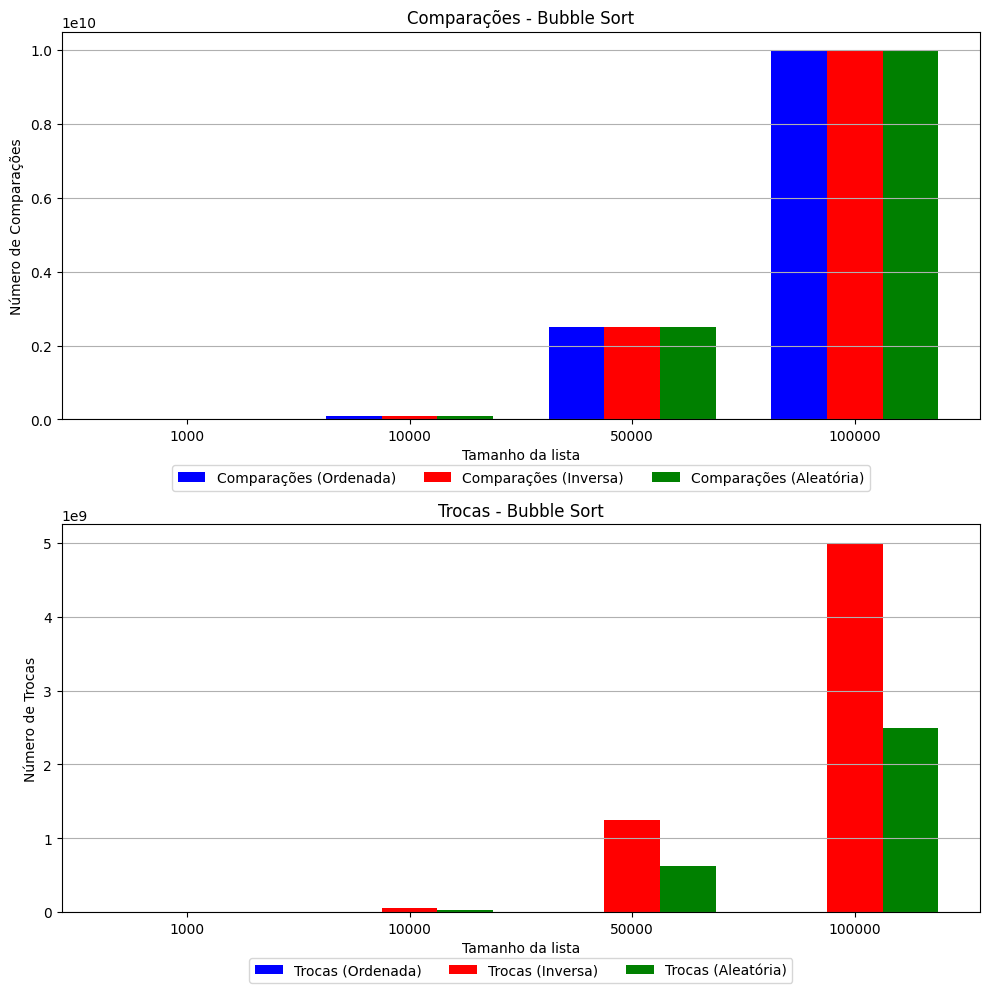
\includegraphics[width=0.5\linewidth]{graficos/grafico_Bubble Sort_comparisons_swaps.png}
    \caption{Bubble Sort}
    \label{fig:bubble-sort}
\end{figure}

\begin{figure}[!h]
    \centering
    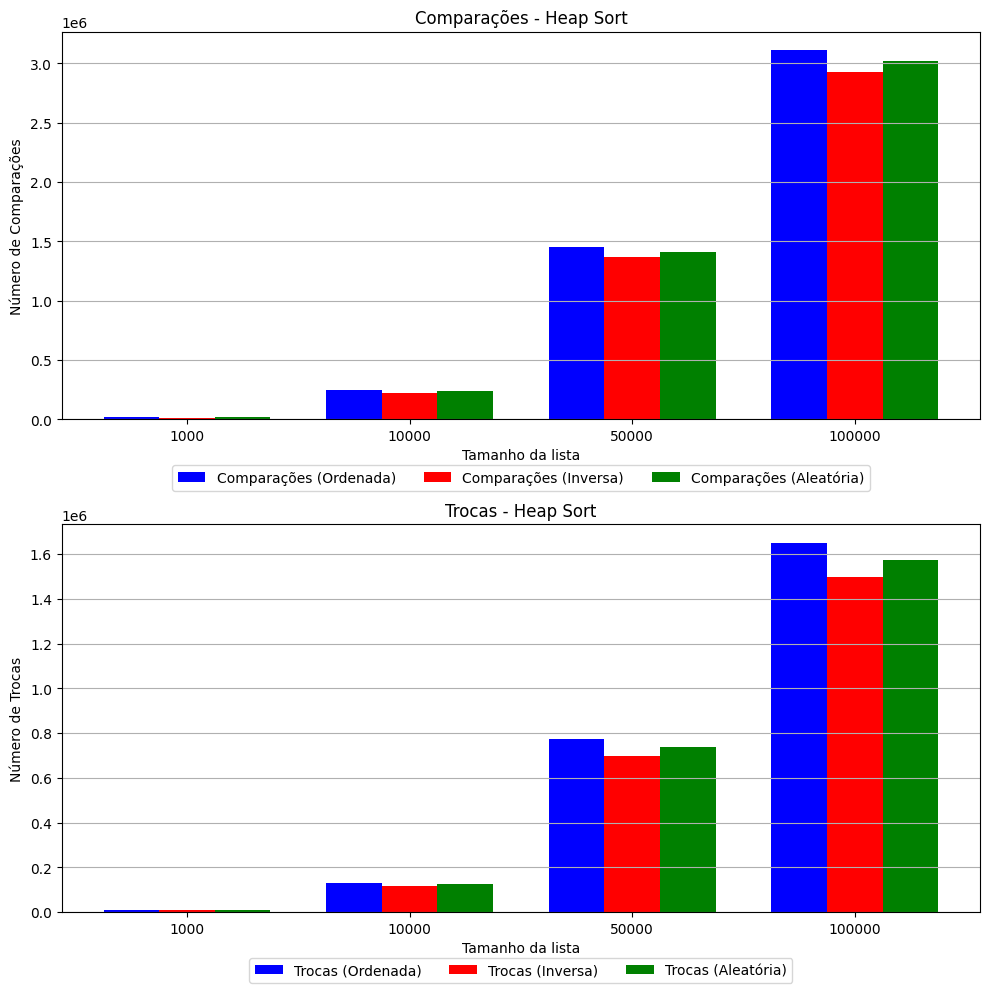
\includegraphics[width=0.5\linewidth]{graficos/grafico_Heap Sort_comparisons_swaps.png}
    \caption{Heap Sort}
    \label{fig:heap-sort}
\end{figure}

\begin{figure}[!h]
    \centering
    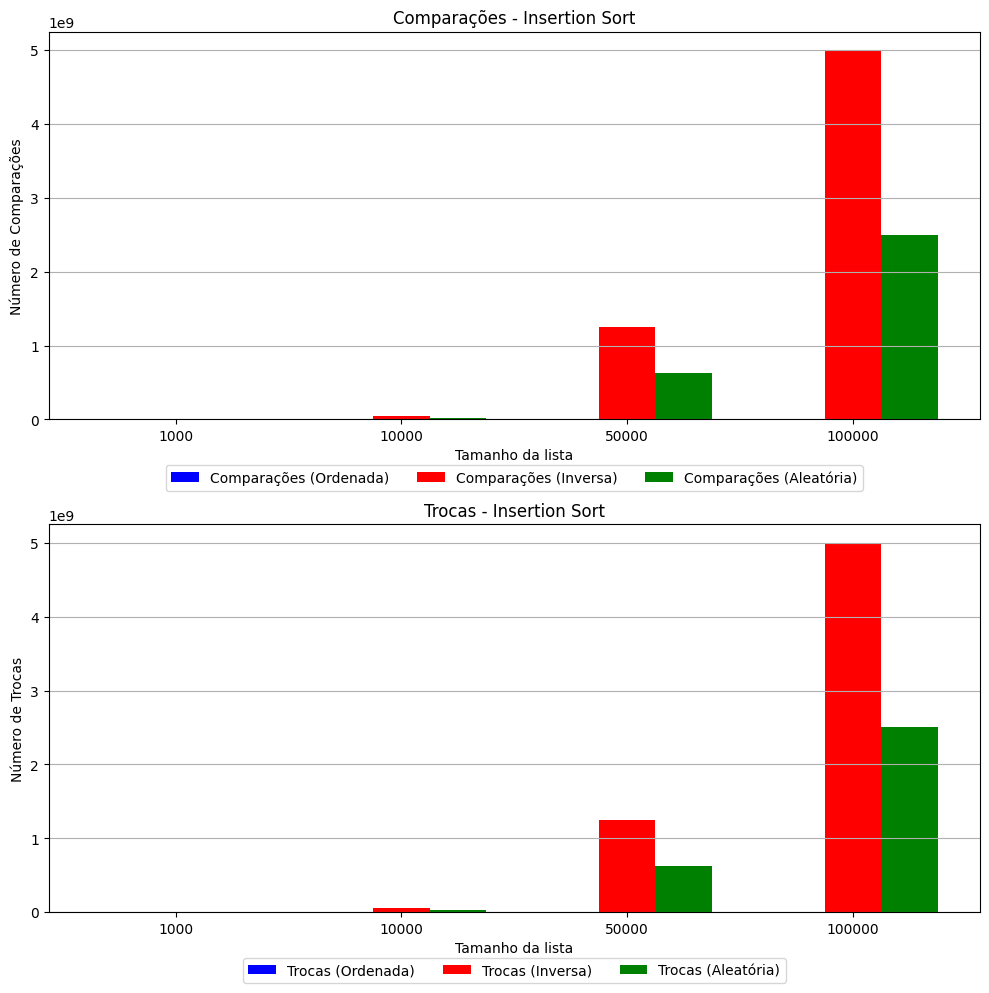
\includegraphics[width=0.5\linewidth]{graficos/grafico_Insertion Sort_comparisons_swaps.png}
    \caption{Insertion Sort}
    \label{fig:insertion-sort}
\end{figure}

\begin{figure}[!h]
    \centering
    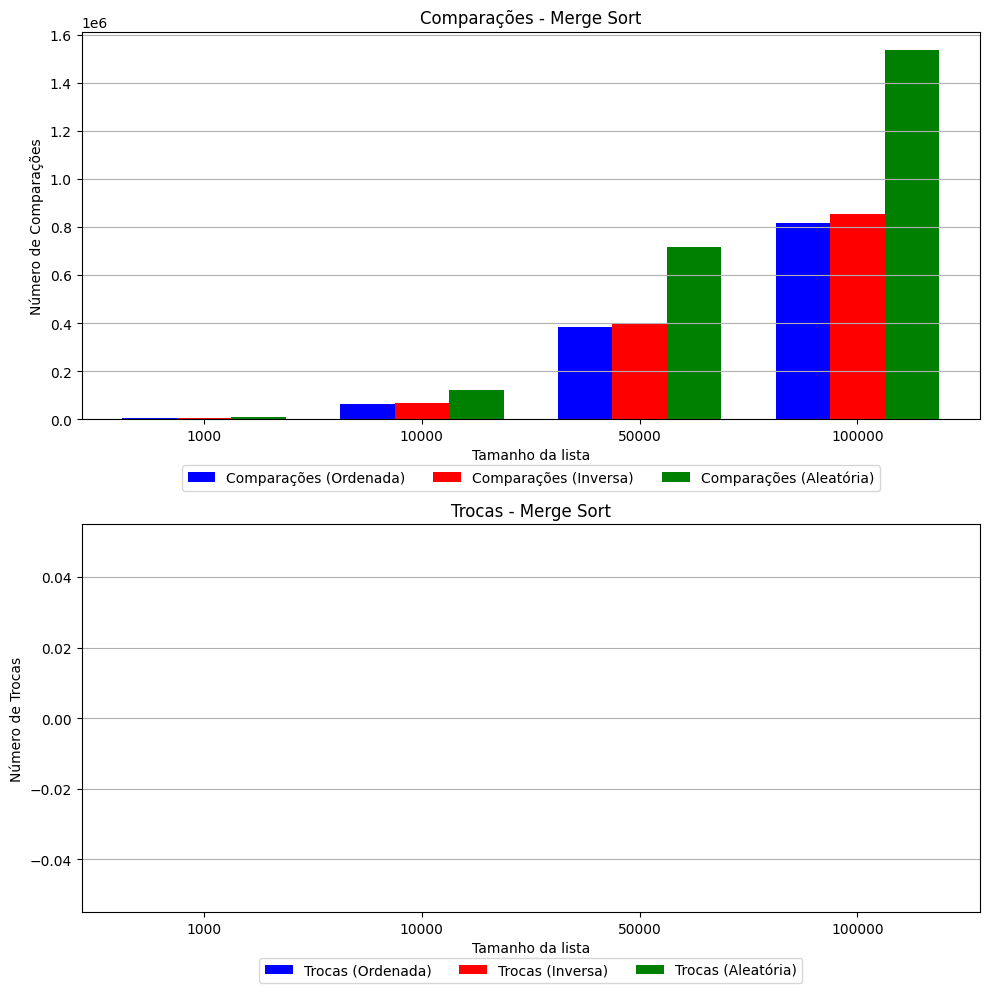
\includegraphics[width=0.5\linewidth]{graficos/grafico_Merge Sort_comparisons_swaps.png}
    \caption{Merge Sort}
    \label{fig:merge-sort}
\end{figure}

\begin{figure}[!h]
    \centering
    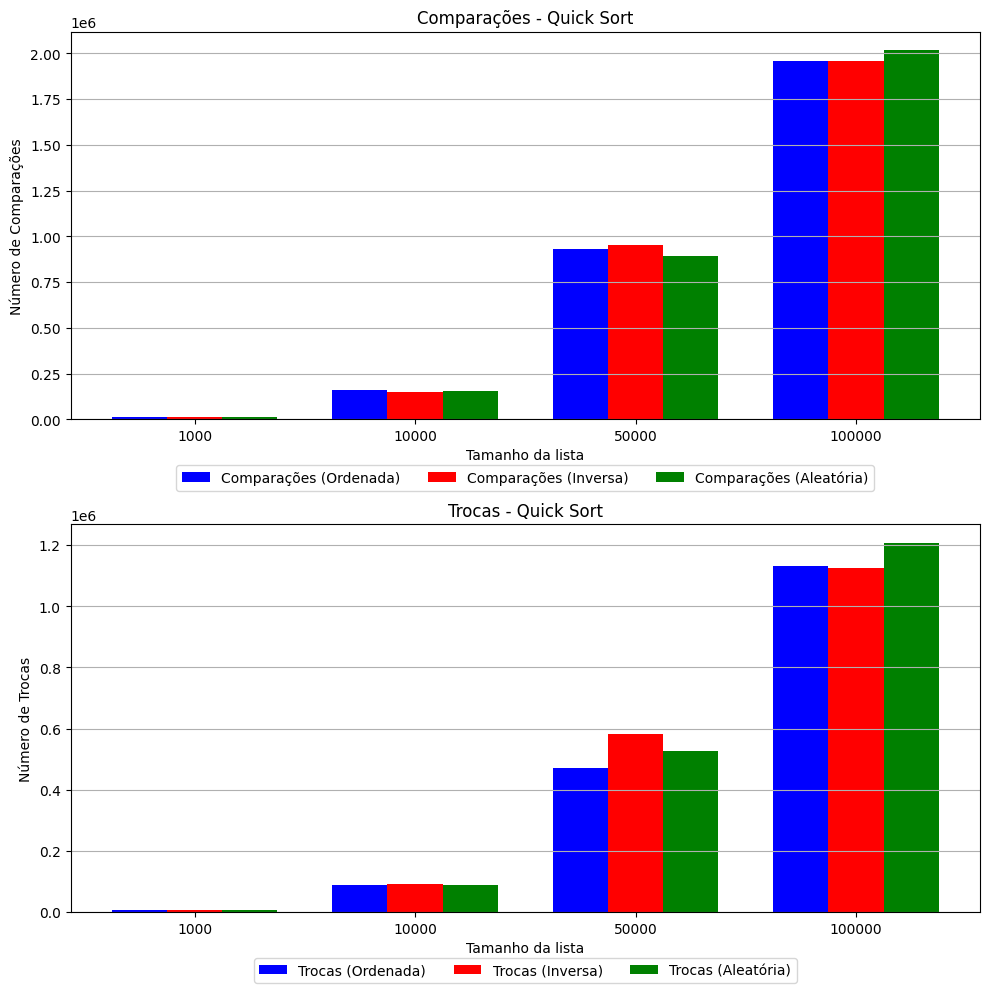
\includegraphics[width=0.5\linewidth]{graficos/grafico_Quick Sort_comparisons_swaps.png}
    \caption{Quick Sort}
    \label{fig:quick-sort}
\end{figure}

\begin{figure}[!h]
    \centering
    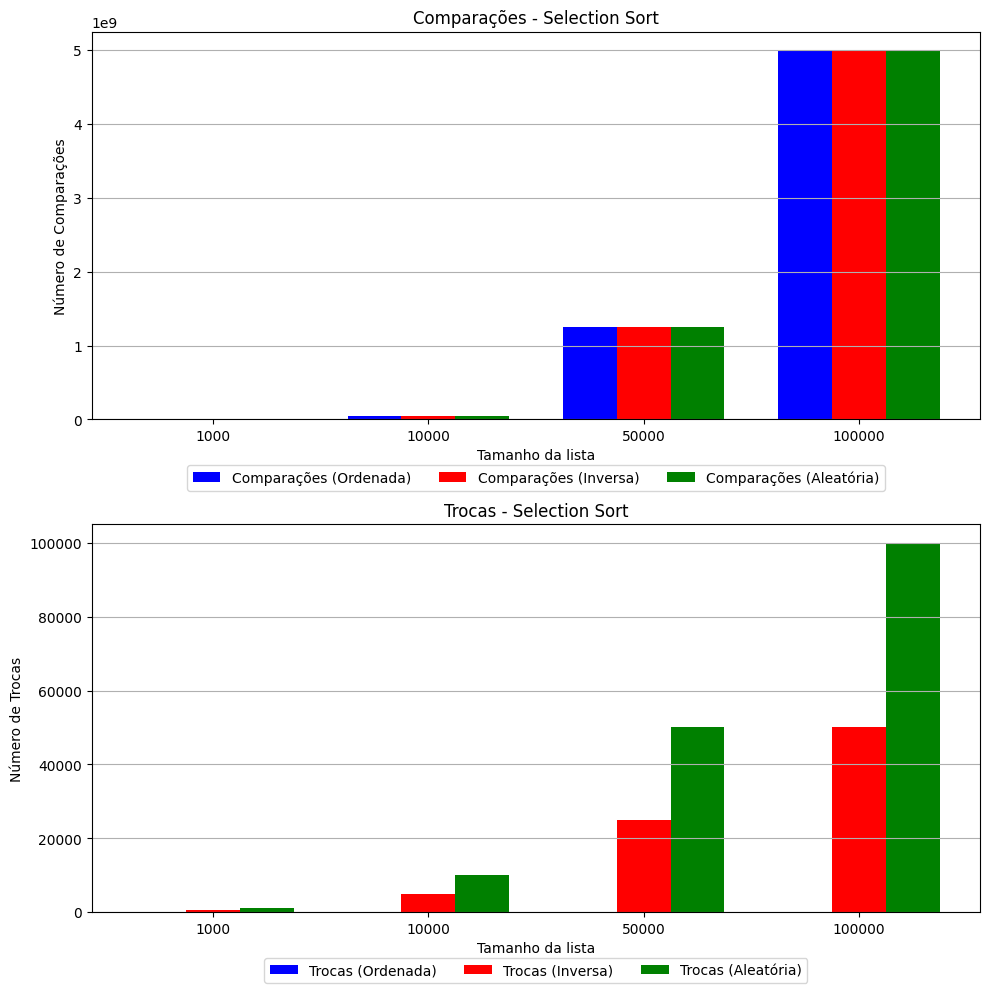
\includegraphics[width=0.5\linewidth]{graficos/grafico_Selection Sort_comparisons_swaps.png}
    \caption{Selection Sort}
    \label{fig:selection-sort}
\end{figure}











\setcounter{figure}{0} % Reinicia a contagem das figuras novamente

\begin{figure}[!h]
    \centering
    
    \subsection{Gráficos que exibem a relação entre quantidade de comparações e de trocas por tamanho da lista, para cada tipo de distribuição.}
    
    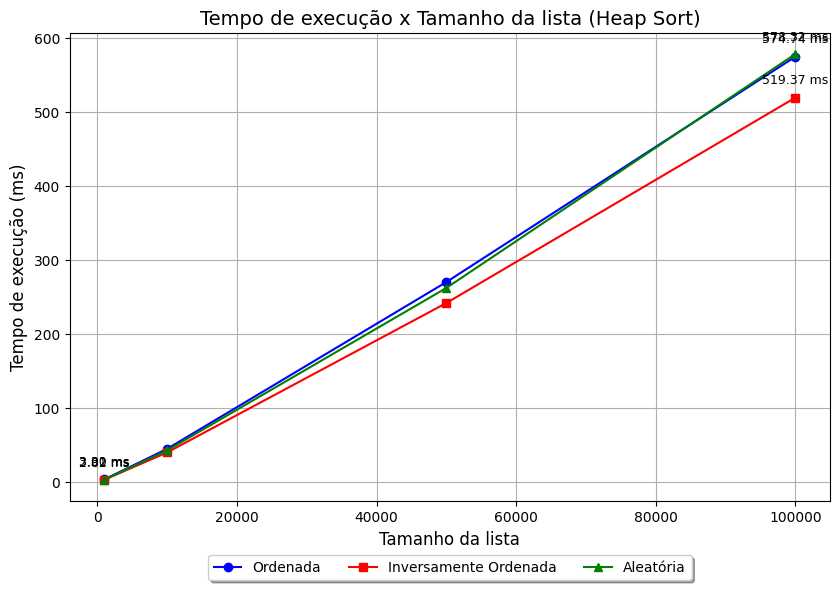
\includegraphics[width=0.5\linewidth]{graficos-tempo/grafico_Heap Sort.png}
    \caption{Heap Sort}
    \label{fig:heap-sort-tempo}
\end{figure}

\begin{figure}[!h]
    \centering
    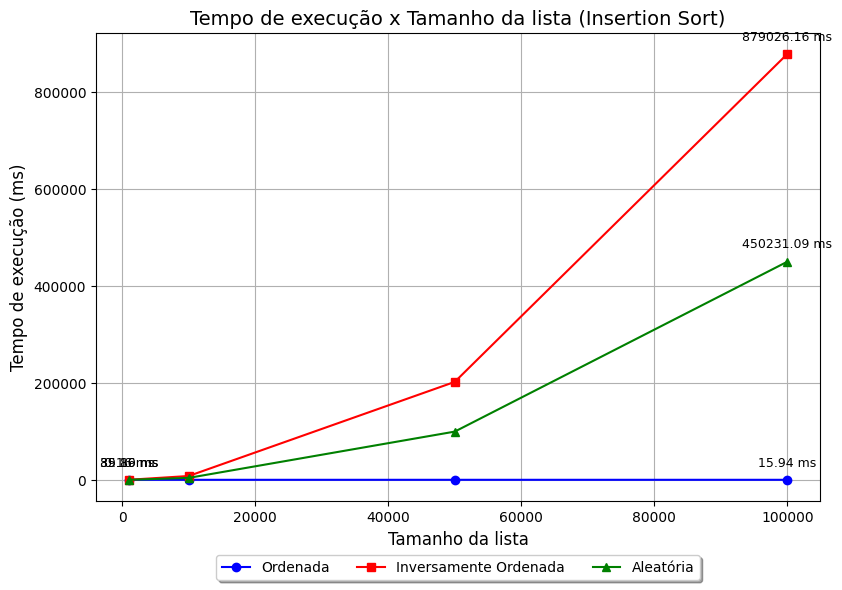
\includegraphics[width=0.5\linewidth]{graficos-tempo/grafico_Insertion Sort.png}
    \caption{Insertion Sort}
    \label{fig:insertion-sort-tempo}
\end{figure}

\begin{figure}[!h]
    \centering
    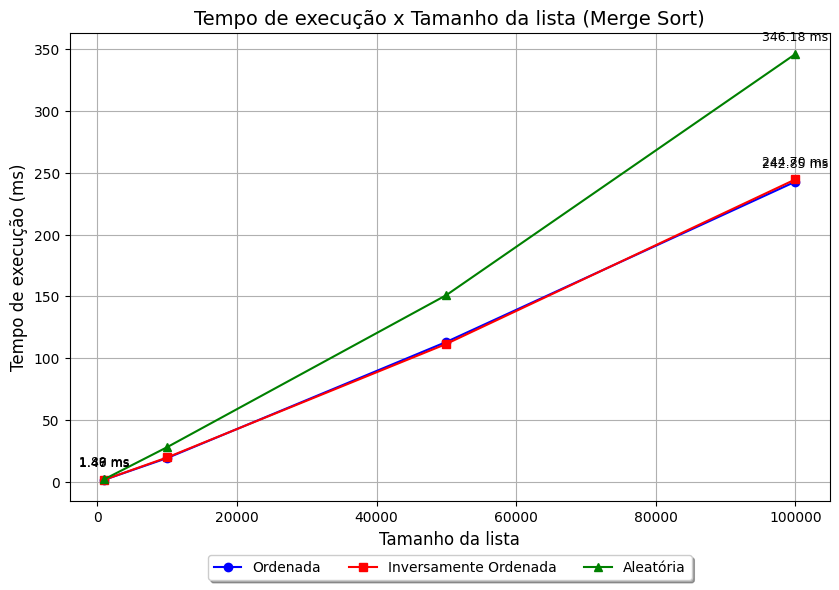
\includegraphics[width=0.5\linewidth]{graficos-tempo/grafico_Merge Sort.png}
    \caption{Merge Sort}
    \label{fig:merge-sort-tempo}
\end{figure}

\begin{figure}[!h]
    \centering
    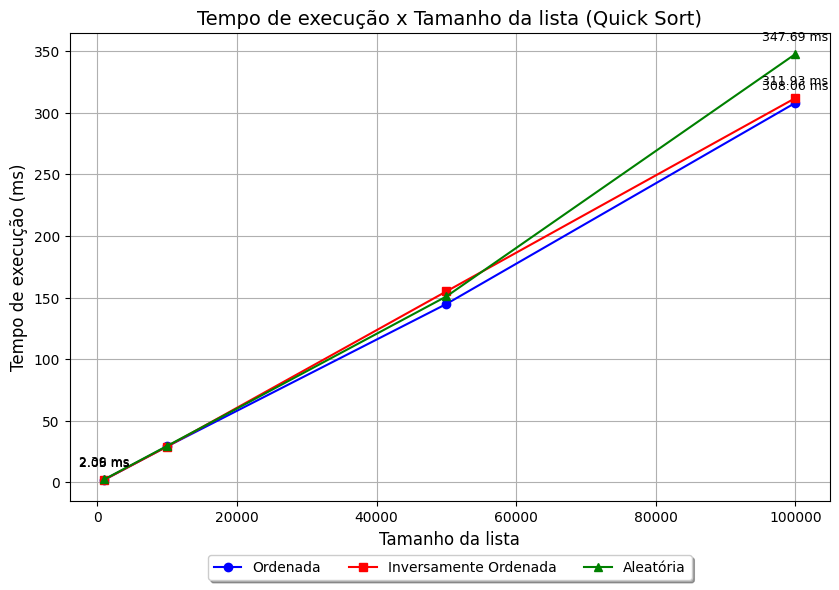
\includegraphics[width=0.5\linewidth]{graficos-tempo/grafico_Quick Sort.png}
    \caption{Quick Sort}
    \label{fig:quick-sort-tempo}
\end{figure}

\begin{figure}[!h]
    \centering
    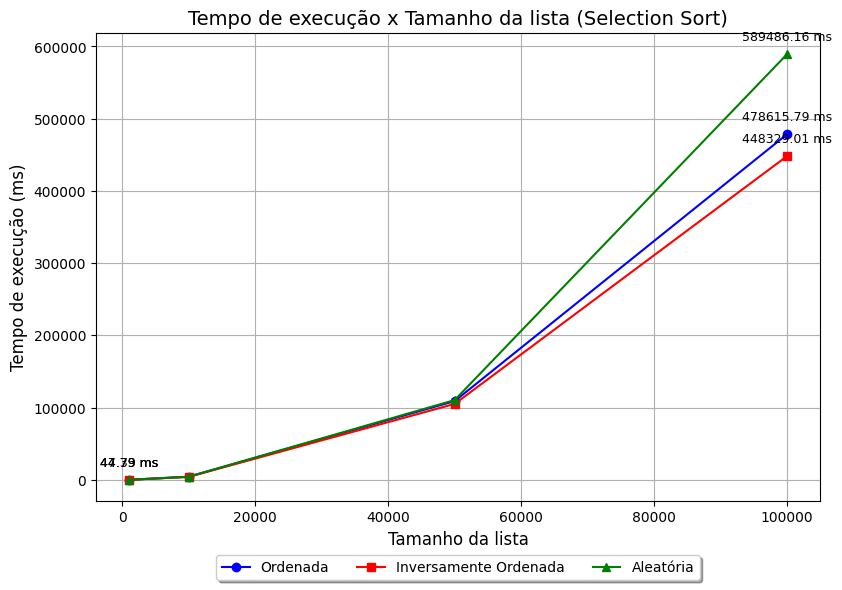
\includegraphics[width=0.5\linewidth]{graficos-tempo/grafico_Selection Sort.png}
    \caption{Selection Sort}
    \label{fig:selection-sort-tempo}
\end{figure}

\begin{figure}[!h]
    \centering
    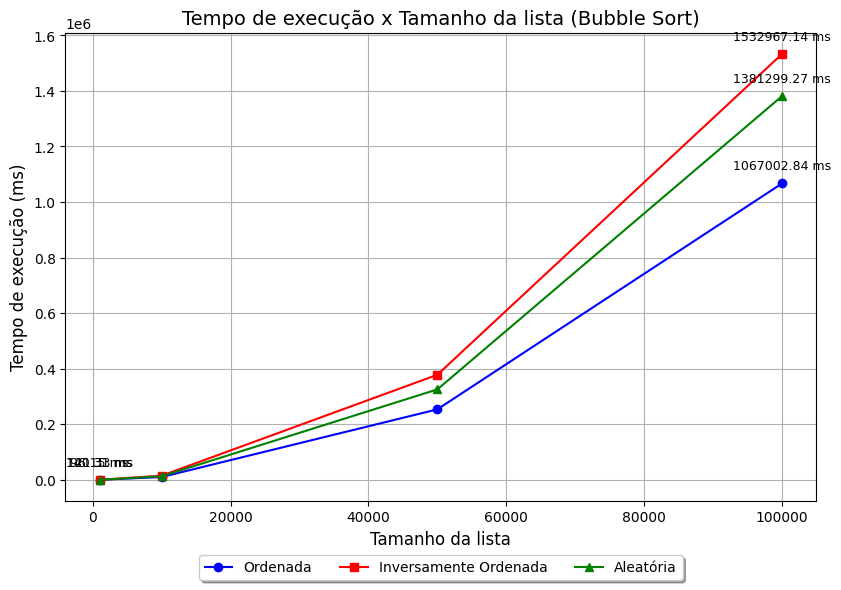
\includegraphics[width=0.5\linewidth]{graficos-tempo/grafico_Bubble Sort.png}
    \caption{Bubble Sort}
    \label{fig:selection-sort-tempo}
\end{figure}


\section{Discussão}

\subsection{Análise dos Resultados}
Os resultados dos experimentos estão em conformidade com a teoria. Algoritmos como Merge Sort e Heap Sort mostraram desempenho consistente com $O(n \log n)$, independentemente da distribuição dos dados. Quick Sort apresentou bom desempenho em listas aleatórias, mas teve uma queda significativa em listas ordenadas ou inversamente ordenadas, devido ao seu pior caso $O(n^2)$. Algoritmos como Bubble Sort e Insertion Sort demonstraram ineficiência em grandes entradas, conforme esperado, devido à complexidade $O(n^2)$.

\subsection{Facilidade de Implementação e Uso de Memória}
Bubble Sort, Selection Sort e Insertion Sort são algoritmos simples de implementar, mas ineficazes em grandes conjuntos de dados. Merge Sort, apesar de eficiente, não é \textit{in-place} e requer mais memória, enquanto Quick Sort e Heap Sort são \textit{in-place}, sendo mais adequados em ambientes com restrição de memória. Apenas Merge Sort e Insertion Sort são estáveis, o que pode ser importante em certas aplicações.

\subsection{Limitações e Sugestões Futuras}
As limitações incluem o uso de uma máquina com especificações fixas, o que restringe a generalização dos resultados. Futuramente, recomenda-se explorar algoritmos paralelos, o impacto de diferentes configurações de hardware e o uso de \textit{datasets} reais. Algoritmos híbridos como TimSort também poderiam ser considerados para uma análise mais abrangente.


\section{Conclusão}

\subsection{Síntese dos Achados}
Este trabalho analisou seis algoritmos de ordenação — Bubble Sort, Selection Sort, Insertion Sort, Merge Sort, Quick Sort e Heap Sort — comparando seu desempenho em termos de tempo de execução, número de comparações e trocas em diferentes cenários de entrada. Algoritmos com complexidade $O(n \log n)$, como Merge Sort e Heap Sort, confirmaram maior eficiência em grandes volumes de dados. Quick Sort mostrou-se eficiente em entradas aleatórias, mas vulnerável a quedas de desempenho em dados ordenados ou inversamente ordenados. Por outro lado, algoritmos quadráticos como Bubble Sort e Selection Sort provaram-se inadequados para listas maiores, sendo úteis apenas em pequenas entradas.

\subsection{Recomendações}
Recomenda-se o uso de:
\begin{itemize}
    \item \textbf{Merge Sort}: quando a estabilidade e a eficiência são críticas, mesmo em ambientes com maior uso de memória.
    \item \textbf{Quick Sort}: ideal para dados aleatórios em cenários onde o espaço de memória é limitado, tomando cuidado com listas quase ordenadas.
    \item \textbf{Heap Sort}: apropriado em situações que exigem eficiência com baixo uso de memória, sem necessidade de estabilidade.
    \item \textbf{Insertion Sort}: útil para pequenos conjuntos de dados ou listas que já estão quase ordenadas.
    \item \textbf{Bubble Sort e Selection Sort}: apenas em contextos educacionais ou para pequenos volumes de dados devido à sua simplicidade e baixa eficiência em grandes entradas.
\end{itemize}

\bibliography{projeto_exemplo}

\end{document}